\section{The Coupled Oscillator}
Consider the system shown in \ref{Fig:CoupledMasses} consisting of two boxes of equal mass $m$ connected by three springs of equal spring constant $k$.  A natural question is, given initial positions and velocities of the boxes at time $t_{0}$ what are their positions and velocities at another time $t$?  To answer this question we have to solve Newton's equation for each box.  This is not so easy.  The equations of motion (Newton's equations) for the boxes are
\begin{equation} \label{eq:Newton}
\ddot{x}_{1} = \omega_{0}^{2} (-2x_{1} + x_{2}) \qquad
\ddot{x}_{2} = \omega_{0}^{2} (-2x_{2} + x_{1})
\end{equation}
where $\omega^{2}_{0} = \frac{k}{m}$.  This is a set of two second order differential equations which are \textit{coupled}, meaning that each equation has dependance on both $x_1$ and $x_2$.  To the untrained eye it looks very difficult to solve.  You are urged to try to solve for $x_{1}(t)$ and $x_{2}(t)$ so that you will appreciate the power of what is to come.

\begin{figure}
\begin{centering}
\includegraphics[width=12cm]{boxes.pdf}
\par\end{centering}
\caption{Coupled mass system. Each spring has spring constant $k$ and each box has mass $m$. The walls are fixed in place.}
\label{Fig:CoupledMasses}
\end{figure}

\begin{flushleft}\textbf{Exercises}\end{flushleft} %Exercises
\begin{itemize}\item[1)] Verify that (\ref{eq:Newton}) correctly describes the motion of the two coupled masses.\item[2)] Try to solve for $x_{1}(t)$ and $x_{2}(t)$.\end{itemize}
